\chapter{Alignment with repeats}

\section{Tandem Repeats}
Tandem repeat is a region in the gnomic sequence that contain two or more
consecutive repetitions of the same sequence. After this evolution event
occurred, mutations, insertions and deletions could happened so the repetitions
seen in current sequences are not necessary exact. This occurs when ??.\todo{Ako sa stavaju repeaty}
Tandem repeats causes problem in the alignment

\begin{reformulate*}
Tu chcem popisat co su to repeaty, ake problemy mozu robit v zarovnani (nejake
priklady) a podobndde.
Presnejsie: \\
$*$ Co je tandem repeat\\
$*$ Priklad tandem repeatu\\
$*$ Ako vznikaju\\
$*$ Priklad zarovnania aj s problemovym tandem repeatom a problemom ako to zarovnat

\end{reformulate*}
\section{Finding repeats}
\begin{reformulate*}
Popiseme ako sa daju hladat repeaty, napriklad aj nasim jednoduchym modelom,
alebo napriklad aj tandem repeat finderom.
Presnejsie:\\
$*$ Tandem repeat finder\\
$*$ TANTAN\\
$*$ SUNFLOWER model \\
$**$ Najskor taky pekny s cyklom \\
$**$ Potom taky menej symetricky, ale bez cyklu \\
$*$ Kontextove gramatiky?
$*$ Repeat masking
\end{reformulate*}
\section{Models}

\begin{reformulate*}
Popiseme nase oba modely. sunflower, a ten tantan-like
Presnejsie:\\
$*$ Ake zhruba ciele mame (mozno do inej kapitoly)\\
%$*$ Popisat to ako 4-stavovy generalizovany model\\
%$*$ Instancia ako SUNFLOWER\\
%$*$ Instancia ako TANTAN\\
%$*$ Expandovanie ciernej skrinky
\end{reformulate*}

In this section we describe models that we have used in our methods. We
describe it in an dual way. As an generalized PHMM and later we extend it into
equivalent PHMM (emissions length are at most $1$ in all sequences).
Equivalency is in the way, that distribution of generated alignments and
annotations are same.

Generalized model is obtained by taking simple three state HMM model from
section \ref{} and adding single generalized pair state $R$, called
\firstUseOf{repeat state}, that in single step generates whole tandem repeats
in both sequences. Since $R$ state can in theory generate arbitrary long
sequences, while decoding using this model, $R$ state does not produce
alignment of bases of tandem repeats. Its aim is to filter tandem repeats out
of alignment so that they do not cause biases in the alignments formed by other
states (match and indel states). To realign those parts later in
post-processing step. The overall topology of GPHMM is illustrated in figure
\ref{FIGURE:REPEAT_GENERAL}.

To made this model flexible, emission distribution of $R$ is defined by
additional PHMM. Since repetitive sequences in tandem repeat are very similar
to each other, we did not try to model the evolution of repetitive part of the
sequence. We assumed that repeats generated by one emissions of $R$ originates
from single consensus sequence and were developed independently. Model was
constructed from sunflower models. Let $C$ be the set of all consensuses that
we want to model. For each consensus $c\in C$ we created sunflowers $S_c^X$ and
$S_c^Y$.  $S_c^X$ is pairwise sunflower model with consensus $c$ that generates
symbols in sequence $X$ and nothing in second sequence. $S_c^Y$ is analogous.
We connect $S_c^Y$ after $S_c^X$ and thus getting model $H_c$ that generates
repeats in both sequences. We connected models $H_c$ for $c\in C$ in parallel
by single start and single end state as in figure \ref{FIGURE:REPEAT_GENERAL}.
The probability from start state to model $H_c$ was determined from posterior
distribution of consensuses $\prob{c}$. Note that the size of this model is
determined mostly by the size of set of all consensuses and therefore this
model can be very large, even infinite if we consider all possible sequences as
an possible consensus for an repeat. To keep the model size small we used
program TRF to compute a set of candidate consensuses $C$ and use it for
construction of model.  We call this generalized model \abbreviation{sunflower
field}{SFF}.

\begin{figure}
\begin{center}
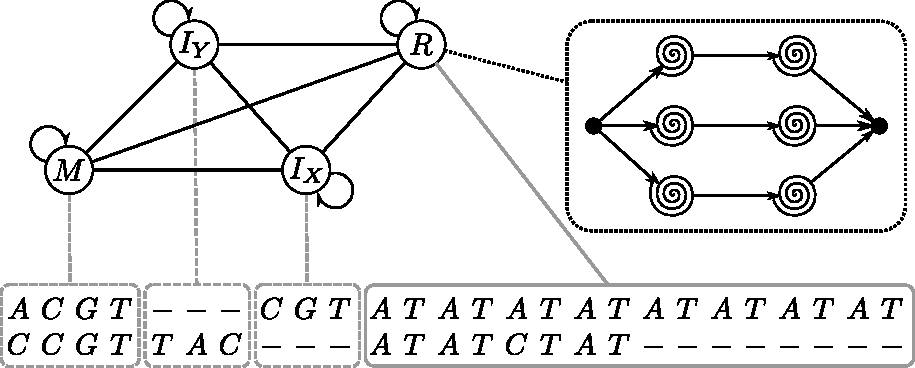
\includegraphics[width=14cm]{../figures/PairRepeatHMMGeneral.pdf}
\end{center}
\caption[General topology of Repeat PHMM]{ 
Topology of Repeat PHMM. We extend 3-state PHMM with one generalized states
$R$, that in one emission generates tandem repeats in both sequences. The
emission distribution of $R$ state is defined by another PHMM. Gray lines
represents emissions: dashed lines corresponds to multiple emissions from same
states, while full line represents one emission. Dotted black line represents
connection to submodel that is used for generating tandem repeats.

Black states in submodel on the right are silent start and end states. Spirals
represents submodels generating tandem repeat in one sequence. They are in
pairs of two identical models, one for generating tandem repeat in one
sequence, other for generating tandem repeat in other sequence. There are
multiple pairs of submodels, each for modeling different consensus.

 }\label{FIGURE:REPEAT_GENERAL} 
\end{figure}

We also experimented with using TANTAN-like model in construction of PHMM
defining emissions distribution of state $R$. Since TANTAN model does not model
the first repetition, we have added chain of states $I_1, \dots, I_n$ to model
first repetition.  Similarly as with sunflowers, we created two copies of
TANTAN, each generating repeats in only one sequence and connect them together
exactly as we would connect sunflowers. Since TANTAN model does not rely on
consensus, it is not necessary to create more copies of TANTAN HMM and it's
general topology looks like SFF's with only one consensus. Since TANTAN is high
order HMM, resulting model is high order and generalized pair HMM. We refer to
this model as \abbreviation{TANTAN PHMM}{TTP}. Advantage of this model over SFF
is in it's size, since TTP will have in practice less states than SFF. However
in TTP, does not satisfy assumption that repeats origins from single consensus,
since each repetitive element is created from previous occurrence and repeats
in sequences $X$ and $Y$ are independent of each other. \todo{obrazok?}

While having SFF or TTP defined as an $4$ state hight order GPHMM might be
convenient for some decoding methods, in general using generalized models
increase time complexity of decoding algorithms quadratically. Therefore we
also worked with their expanded versions: we removed state $R$ and replace it
with model generating repeats (referred as a submodel). All transitions
entering originally into $R$ were directed to start state of submodel and all
outgoing transitions from $R$ now start in end state of submodel. Distributions
of alignments generated by this PHMM has clearly not changed. Additionally, if
in original GPHMM we used identity function as an labeling function
$\lambda_{ID}$ and in expanded model we label states from submodel by label
$R$, resulting in labeling function $\lambda_R$, distribution on annotations
on alignments has also not changed. \todo{toto znie ako od hotentota}


\begin{comment}
By this we obtained model that 

We started from HMM $H$ that model repeats and alter it to
PHMM, so that it generates empty sequences in one strand. By this we get 2 HMMs
$H_X$ and $H_Y$, first that generates bases only in sequence $X$ and second
that generates bases only in sequence $Y$. 

tandem repeats together, just label them that they 
\begin{itemize}
\item Reduce alignment alignment error near repeats
\item Improve alignment of the repeats
\end{itemize}
We kept in mind following \reformulate{???} while designing model:
\begin{itemize}
\item We assume star phylogeny of the repeats: all repetitions of repeat evolved
from single consensus sequence independently.
\item We want to label repetitive regions.
\item Correct alignment of two repetitive regions is very hard, if not
impossible. This is because these regions are very similar \todo{Chcelo by to
vygenerovat graf, sekvencnej identity, poctu insertov a podobne ako funkciu vo
vzdialenosti od repeatu}.
\end{itemize}


We have two models, sunflower and TANTAN-like model. They both differ
significantly in how they treat consensus.

The main model is similar to standard 3-state model for pair alignments. We
have added  submodel modeling repeats. All states in the submodel had same
label. Repeats were modeled in each sequence independently, so basically to
model repeats, we have chained model for repeats in sequence $X$ and model for
repeats in sequence $Y$. We did not try to model evolution of the repeats due
to the high sequence similarity of repeats.  We do not believe that there is
enough information in the repeats (and errors in them) to practically improve
the alignments of the repeat parts. On the other hand, this model produces
alignments where all repetitions were indels, which is not realistic. To cope
with this drawback, we realigned repetitive parts along with flanking
insertions by simple 3-state HMM.

While the TANTAN model models repeats of any sequences, we could just have one
copy of TANTAN model for sequence $X$ and one copy for sequence $Y$.  However,
for the sunflower submodel, each sunflower models only repeats of one specific
sequence, therefore we can model only one possible repetitive sequence by using
only one\footnote{Two same sunflowers for both sequences.} sequence. To
overcome this very strict constrained, we have to one sunflower per consensus
we want to model. We put sunflowers together in parallel way, so that they are 
Topology of both of these models are described in figure \ref{}.

\end{comment}

\section{Decoding methods}
\begin{reformulate*}
Tu popiseme ake dekodovacie metody pozname: viterbi, posterior, block \{viterbi,
posterior\}
Presnejsie:\\
$*$ Viterbi\\
$*$ Posterior (marginalized aj nie)\\
$*$ Block viterbi\\
$*$ Block posterior\\
\end{reformulate*}
\section{Implementation details \& optimizations}
\begin{reformulate*}
Implementacne detaily, optimalizacie, cachovanie
Presnejsie:\\
$*$ Banding, \\
$*$ Konsenzy -- TANTAN vs SFF\\
$*$ ako sa cachovali, spomenut ze ake rozne optimizacne kriteria by to mohlo mat\\
$*$ Ako sa vyberali hinty pre block viterbi
\end{reformulate*}
\section{Experiments}
\begin{reformulate*}
Ako sa generovali data, ako sa trenovali modely, ake miery sledujeme
\end{reformulate*}
\section{Results}
\begin{reformulate*}
Tabulky, grafy, ...
\end{reformulate*}

\section{Possible Improvements}

\begin{reformulate*}
Sem by som mohol napisat, ako by sa dal pouzit symetricky model s cyklom
stavov, alebo ako by sa dal ten cyklus stavov odstranit odstranenim jednej
hrany a pridanych n hran -- co je lepsie ako pridat n vrcholov.
\end{reformulate*}

\label{LastPage}
